\chapter{Experiments}
\label{chap:experiments}

This thesis proposes a manipulation planning approach targeted
at coupled multi-step problems under resource constraints,
as formulated by Chapter~\ref{chap:formulation}.
In order to evaluate the efficacy of the approach,
this chapter details a set of experiments on multiple robot systems
both in simulation and on real hardware.

While we focus here on a comprehensive evaluation of our algorithms
on multi-step problems with high-DOF robots,
we also point the reader to the targetted empirical evaluations
performed for each algorithm individually:
\begin{itemize}
\item The comparison of the E$^8$ graph search algorithm to
   weighted and anytime alternatives in Chapter~\ref{chap:e8}.
\item The comparison of the E$^8$-PRM roadmap planner to
   other state-of-the-art single-query algorithms in
   Chapter~\ref{chap:graphs-in-continuous}.
\item The comparison of the Multi-Set PRM roadmap planner to
   alternative approaches, such as Experience Graphs,
   using a simple sequential task planner
   in Chapter~\ref{chap:multi-set-prm}.
\end{itemize}

This chapter describes the test platforms,
metrics,
control variables,
and baseline approaches that are used in the experimental
evaluation.
We then detail each experiment in detail
and present the results obtained.

\section{Test Platforms and Software Framework}

We used the following two robot systems for our evaluations.

\begin{figure}
{\setlength{\offsetpage}{0.5in}
\begin{widepage}
   \centering
   \begin{subfigure}[t]{0.48\textwidth}
      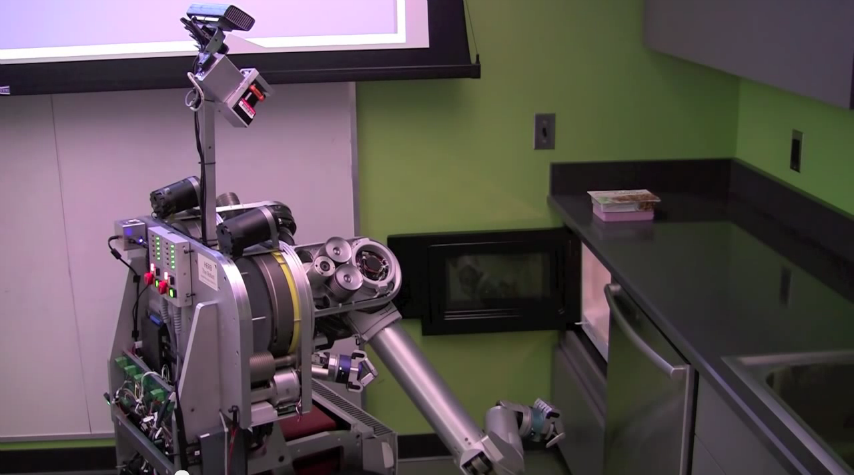
\includegraphics[width=\textwidth]{figs/herb-microwave-intro.png}
      \caption{The \textsc{Herb} assistance robot
         must move a frozen meal into a microwave oven.
         \cdnote{Add clutter.}}
      \label{fig:exp-platforms-herb}
   \end{subfigure}%
   \quad%
   \begin{subfigure}[t]{0.48\textwidth}
      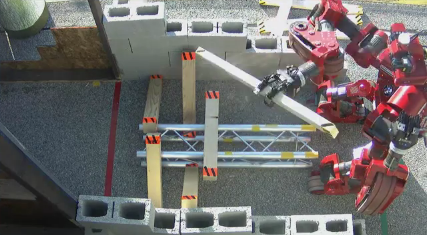
\includegraphics[width=\textwidth]{figs/chimp-debris-overhead.png}
      \caption{The \textsc{Chimp} distaster response robot
         must clear large pieces of debris from a blocked doorway.}
      \label{fig:exp-platforms-chimp}
   \end{subfigure}
   \caption{The two hardware platforms used for experimental
      results.}
   \label{fig:exp-platforms}
\end{widepage}
}%offsetpage
\end{figure}

\subsection*{HERB: The Home Exploring Robot Butler}

The HERB robot \cite{srinivasa2012herb20},
Figure~\ref{fig:exp-platforms-herb},
is human-scale mobile manipulator designed to assist in home
environments.
It has two seven-degree-of-freedom Barrett WAM arms mounted
on a Segway RMP base.
It includes a BLAH KWh battery and has three onboard rack-mount
computers.

\subsection*{CHIMP: the CMU Highly Intelligent Mobile Platform}

CHIMP \cite{stentz2014chimp},
Figure~\ref{fig:exp-platforms-chimp},
is a disaster response robot built by NREC at CMU
for the Darpa Robotics Challenge.
It is a tracked mobile manipulation robot consisting of
four limbs comprising 26 limb degrees of freedom.
It has Robotiq adaptive 3-finger grippers.

\subsection*{OpenRAVE Simulation Environment}

We use the OpenRAVE \cite{diankov2010openrave} simulation environment
for planning and collision checking.
It implements kinematics, robot models,
and interfaces to several collision checkers.
When reporting planning effort,
we present both total time and energy used,
as well as number of collision checks performed
for comparison to other checkers.
See the section on metrics below.

\subsection*{Open Motion Planning Library}

We use the Open Motion Planning Library (OMPL)
planning framework \cite{sucan2012ompl}
to implement our planners
and for baseline approaches which we compare against.

\section{Metrics}

In order to conduct a fair experimental comparison,
we describe here the metrics we collect for each approach.

Our primary metric is \emph{total task effort} exerted to accomplish
the task.
For each run of our algorithms,
we record this effort as measured in
(a) time, in seconds,
and (b) energy, in Joules.
In order to present these data as fairly as possible,
we record the split between planning and execution effort
for each plan.
We also report the difference between expected and actual
execution effort for the solution path
that may result from an approximate execution effort model
(see Chapter~\ref{chap:graphs-in-continuous}).

To enable comparisons to other robots and collision checkers,
we also report number of collision checks as a proxy for collision
checking effort.
We also report the number of triangles in each collision model.

Because our method (and those we compare against)
are inherently probabalistic,
we perform each experiment on multiple different graphs,
and report summary statistics.
For a full picture,
we present full cumulative probability distributions
for total task effort across all runs of each planner.
We also present median and mean results for comparison.

While our approach terminates automatically
given an the input $\lambda$ parameter between planning and execution
effort,
we also compare against anytime approaches that return multiple
improving solutions over time.
We present plots of all of these results for comparison,
and also report the data points that result from several
a-priori time budgets.

\section{Control Variables}

Our approach takes explicit advantage of several aspects of the
structure of multi-step manipulation planning problem
in order to perform efficiently.
In order to evaluate the effects of each of these insights,
we control several continuous and categorical
parameters and factors in our evaluation.
We have several hypotheses which relate these parameters to
the results we expect,
as outlined in the research questions in Chapter~\ref{chap:proposed}.
The control variables we propose to vary are:
\begin{itemize}
\item The $\lambda$ parameter of E$^8$ search
   which mediates between planning and execution effort.
\item The batching approach of the E$^8$-PRM
   which approximates the spatial correlation in
   $\mathcal{C}_{\mbox{\scriptsize free}}$.
\item What kind of multi-set structure is exploited.
   Sometimes, we don't tell the Multi-Set PRM anything about the
   structure between problems.
\item With and without pre-caching.
   Fully known worlds.
   Idle robots?
\end{itemize}

For a fair comparison,
we also select parameters for other approaches using a set of testing
problems.

\section{Baseline Approaches}

We propose to test our task planner against a suite of
state-of-the-art approaches,
including:
\begin{itemize}
\item Hierarchical task and motion planning in the now
   \cite{kaelbling2011inthenow}.
   Note that we compare against HPN both
   interleaved and non-interleaved.
\item The seqeutial task planner used by by the CMU team
   at the Darpa Robotics Challenge
   \cite{dellin2014drc},
   based on the Constrained Bi-Directional RRT
   \cite{berenson2009manifolds}.
\item Other hybrid symbolic/geometric planners.
   \cdnote{Talk to Evan.}
\end{itemize}

\section{Primary Planning Comparison}
\label{sec:exp-noninterleaved}

Isolate planning (no interleaving).

See Section~\ref{sec:exp-interleaved}.

Fixed resolution for validating paths.

Addressing fully known and fully unknown worlds.

Multiple task descriptions.
Microwave and debris.

Also, this is relevant if actions cannot be undone.

\subsection{DRC Experiments (Real Competition Data)}

\subsection{HERB Experiments}

\section{Secondary Comparison with Interleaving}
\label{sec:exp-interleaved}

The Multi-Set PRM handles interleaved planning and execution
because the start nodes can be moved.
We will implement a very simple interleaved version of Proteus
for comparison with interleaved task planning approaches
such as HPN.

Allowing interleaved planning and execution
on deterministic, reversible worlds.
We expect planners like HPN to get a speedup
due to pipelining.
